\subsection*{5.1 Overview}

Flow chart of compiler architecture :

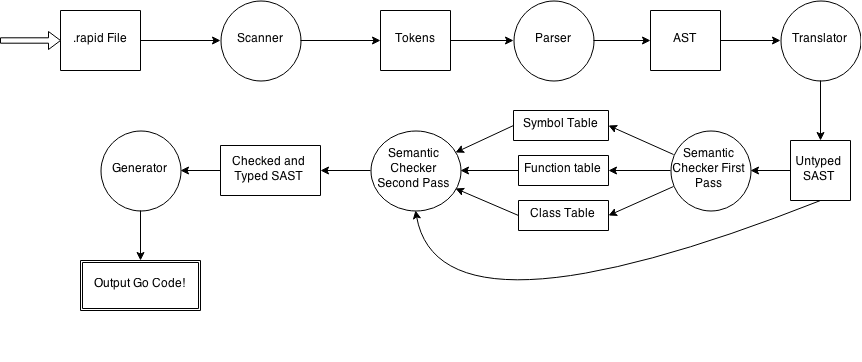
\includegraphics[scale=0.5]{arch_flow.png}

The compilation of Rapid to go is broken down into 5 stages:

\begin{enumerate}
\item Scanning
\item Parsing
\item Translating
\item Semantic Checking/Type Checking
\item Code Generation
\end{enumerate}


\subsection*{5.2 Scanning}

The scanner is written in \textbf{ocamllex} and takes a .rapid text file and converts it into a stream of tokens.  The tokens represent keywords, types, and identifiers in the rapid program.

\subsection*{5.3 Parsing}

The parser uses \textbf{ocamlyacc} to convert the tokens it receives from the scanner into and abstract syntax tree (AST).  The parser builds the AST as a list of statements, functions, classes and http trees.  Statements hold the kind of statement and associated expressions.  Functions hold a their name, a list of statements representing the variable declarations for the arguments, a list of statements representing the body and a list of statements. A class declaration has a list of it's members (Attributes or Functions). Finally an Http is a recursive tree here each no leaf node of the tree is a namespace block or a param block.  The leaves of the tree are http functions.  

\subsection*{5.4 Translation}

Translation gets the AST from the parser in the from of a tuple of AST Statements, AST Functions, AST HTTP trees and AST Classes.  Translation takes the AST and Translates it to an initial semantic abstract syntax tree (SAST). This SAST has the same structure as the AST.  At this step all literals are rewritten to typed expressions.  

\subsection*{5.5 Semantic Checking}

After translation the SAST is scanned for variable declarations, function declarations, and class declarations.  When one of these is found it is added to the symbol table, function table, or class respectively.  This pass must be done before semantic checking because functions and class do not have to be declared before being used.  Once these tables are built the SAST is walked once more to check types.  Expressions are recursively rewritten to typed expressions and then typed checked. In binary operations ints are marked for casting to float if they are found in a binary operator expression expecting a float.  Functions declarations are scanned for a return statement of the proper type.  Statements are check to make sure their expressions are of the correct type.  Class instantiations and function calls are check for the proper number and type of arguments they are passed.  Once all this type checking and rewriting is done the SAST is passed to the code generator.

\subsection*{5.6 Code Generation}

The code generator takes the SAST from the Semantic Checker and generates go code.  Because go has a main function and RAPID does not, we first pull out all the var declarations and write the go declarations before main. This is because these variables are global in our language. Now we recurse through each part of the SAST (statements, functions, classes, and http blocks) and write each part of them to code.  Because our language supports null values and go does not we use go pointers to represent all of our types.  This means that to generate functioning code statements have to be written in two parts.  First, temp variables are created in go and set to value of on part of the expression.  Then these temp values are used to evaluated the expression.  for example rapid code:
\begin{verbatim}
int x = 5; would get 
int i = x;
\end{verbatim}

Would generate the following go code:
\begin{verbatim}
//declartions pulled out
x Int //Int is type we defined as pointer to int.
i Int
//int x = 5; 
tmp = 5
x = &tmp
//int i = x;
tmp = *x
i = &tmp
\end{verbatim} 
